\documentclass[a4paper]{article} \usepackage[backend=biber, style=numeric, sorting=none]{biblatex}
\usepackage[a4paper, left=0.8cm, right=0.8cm, top=0.8cm, bottom=0.8cm, landscape]{geometry}
% \usepackage{showframe}
\usepackage{multicol}
\usepackage{blindtext}
\usepackage{listings}
\usepackage{graphicx}
\usepackage{enumitem}
\graphicspath{{images/cs2100/}}

\begin{document}
\setlength\parindent{0pt} %TODO this somehow messes up paragraph vertical spacing as well?
\scriptsize
% \tiny
\pagenumbering{gobble}

\begin{center}
{\large CS2100 Cheatsheet 17/18 Sem 2}\\{by vig}
\end{center}
    \begin{multicols*}{4}

% NUMBER SYSTEMS & DATA REPRESENTATION %
{\small\textbf{Number Systems \& Data Representation }}
\textbf{Sizes of data/types}
\begin{itemize}[leftmargin=*]
\itemsep -0.5em
\item byte : 8 bits 
\item nibble : 4 bits (half-byte)
\item word : multiple bytes (1, 2, 4) (for MIPS it's 4)
\item \texttt{int} : 4 bytes (1 bit for sign, 31 for magnitude)
\item \texttt{float} : 4 bytes
\item \texttt{double} : 8 bytes
\item \texttt{char} : 1 byte
\end{itemize}

\textbf{Representation \& Complements}
\begin{itemize}[leftmargin=*]
\itemsep -0.5em
\item Convert decimal whole numbers to base $R$ : divide by R, first remainder is LSB, last is MSB
\item Convert decimal fractions to base R : multiply by R, first carry is MSB, last is LSB
\item base ${R}$ to base ${R^N}$: partition in groups of $N$ e.g groups of 4 for base 2 to base 16
\item Convert to R-1s complement : Flip the digits; \texttt{digit = R - digit}
\item Convert to Rs complement : Flip the digits, then add 1 to the number
\item 1s complement has +ive and -ive 0
\item 2s complement has only 1 representation of 0
\item 2s complement can represent an \i{additional} negative number e.g for binary, 1000 represents -8 (+8 cannot be represented in a signed 4 bit number)
\item Convert to excess X: Take number minus X (0 refers to -x)
\item IEEE 754 Floating-Point Representation:  $sign  | exponent  |  mantissa$
\item Single-precision float has 1 bit sign, 8 bit excess-127 exponent, 23 bit mantissa (normalized with a leading bit 1 i.e the mantissa is the X in 1.X)
\item Double has 1 bit sign, 11 bit excess-1023 exponent, 52 bit mantissa 
\end{itemize}

\textbf{Operations with binary numbers}
\begin{itemize}[leftmargin=*]
\itemsep -0.5em
\item 2s complement addition: Simply add \& ignore carry out of MSB
\item 2s complement subtraction: take 2s complement of number to be subtracted, then do 2s addition.
\item 1s complement addition: Add; If there is a carry out, add 1 to the result
\item 1s complement subtraction: take 1s complement of number to be subtracted, then do 1s addition.
\item check for \bf{overflow}: If result is opposite sign of both operands (that have the same sign)
\end{itemize}

% MIPS %
{\small\textbf{MIPS}}

\textbf{R, I, J format}
\begin{itemize}[leftmargin=*]
\itemsep -0.5em
\item $\bf{R}$: $Opcode, rs, rt, rd, shamt, funct$
\item $\bf{I}$: $Opcode, rs, rt, Imm$
\item rd is not used, check datasheet for instruction syntax
\item For branch, $Imm$ is the relative number of \i{words} to go to (with respect to $PC + 4$), in 2s complement representation
\item $\bf{J}$: $Opcode, Address$
\item First 4 bits are assumed to be 4 MSBs of $PC + 4$. Last 2 bits assumed to be 0 (because of word addressing)
\end{itemize}

% Instruction Set Architecture %
{\small\textbf{Instruction Set Architecture}}

\textbf{Architectures \& Endianness}
\begin{itemize}[leftmargin=*]
\itemsep -0.5em
\item Von Neumann: Data(operands) stored in memory
\item Stack: operands are on top of stack
\item Accumulator: One operator is in the accumulator (a special register)
\item Memory-memory (all operands in memory)
\item Register-Register (all operands in registers) (MIPS)
\item Big-endian: Most significant byte stored in lowest address
\item Little-endian: Least significant byte stored in lowest address (easier to read)
\end{itemize}

\textbf{Opcode encoding}
\begin{itemize}[leftmargin=*]
\itemsep -0.5em
\item To maximize, reserve 1 instruction for lesser-bit instruction types.
\item To minimize, reserve all but 1 instruction for lesser-bit instruction types
\item Forumla for maximizing: $2^{no. of bits} * (1 - F)$ where $F$ is the fraction of bits lost by reserving bits
\end{itemize}

% Boolean Algebra %
{\small\textbf{Boolean Algebra}}
\\ \textbf{Laws}
\begin{itemize}[leftmargin=*]
\itemsep -0.5em
\item Identity: $A + 0 = A$ and $A \cdot 1 = A$
\item Complement: $A + A' = 1$ and $A \cdot A' = 0$
\item Commutative: $A + B = B + A$  and $A \cdot B = B \cdot A$
\item Associative: $A + (B + C) = (A + B) + C$ and $A \cdot (B \cdot C) = (A \cdot B) \cdot C$
\item Distributive: $A + (B \cdot C) = (A + B) \cdot (A + C)$ and $A \cdot (B + C) = (A \cdot B) + (A \cdot C)$
\item Duality (not a real law): If we flip AND/OR operators and flip the operands (0 and 1), the boolean equation still holds
\end{itemize}

\textbf{Theorems}
\begin{itemize}[leftmargin=*]
\itemsep -0.5em
\item Idempotency: $X + X = X$ and $X \cdot X = X$
\item One/Zero Element: $X + 1 = 1$ and $X \cdot 0 = 0$
\item Involution: $(X')' = X$ 
\item Absorption: \\ $X + (X \cdot Y) = X$ \\ $X \cdot (X + Y) = X$
\item Absorption (variant): \\ $X + (X' \cdot Y) = X + Y$ \\ $X \cdot (X' + Y) = X \cdot Y$
\item DeMorgans' (can be used on $>2$ variables): \\ $(X \cdot Y)' = X' + Y'$ \\ $(X + Y)' = X' \cdot Y'$
\item Concensus: \\ $(X \cdot Y) + (X' \cdot Z) + (Y \cdot Z) = (X \cdot Y) + (X' \cdot Z)$ \\ $(X + Y) \cdot (X' + Z) \cdot (Y + Z) = (X + Y) \cdot (X' + Z)$
\end{itemize}

\textbf{Minterms \& Maxterms}
\begin{itemize}[leftmargin=*]
\itemsep -0.5em
\item Sum-Of-Products (SOP): Product term or a logical sum of product terms
\item $m$interm: Product term that contains $n$ literals from all the variables
\item Product-Of-Sum (POS): Sum term or a logical product of sum terms
\item $M$axterm: Sum term that contains $n$ literals from all the variables
\item $Mx$ = $mx'$ because of De Morgan's
\item Sum of 2 distinct Maxterms is 1 e.g $M1234 + M1120 = 1$
\item Product of 2 distinct minterms is 0 e.g $m1234 \cdot m1120 = 0$
\end{itemize}

% COMBINATORIAL CIRCUITS %
{\small\textbf{Combinatorial Circuits}}
\\ \textbf{Gates}
\begin{itemize}[leftmargin=*]
\itemsep -0.5em
\item {AND, OR, NOT} is a complete set of logic
\item {NAND} is a complete set of logic
\item {NOR} is a complete set of logic
\item Produce SOP with $AND >> OR$ or $NAND >> NAND$
\item Produce POS with $OR >> AND$ or $NOR >> NOR$
\item With negated outputs, use NAND to simulate OR and NOR to simulate AND
\end{itemize}
{\centering 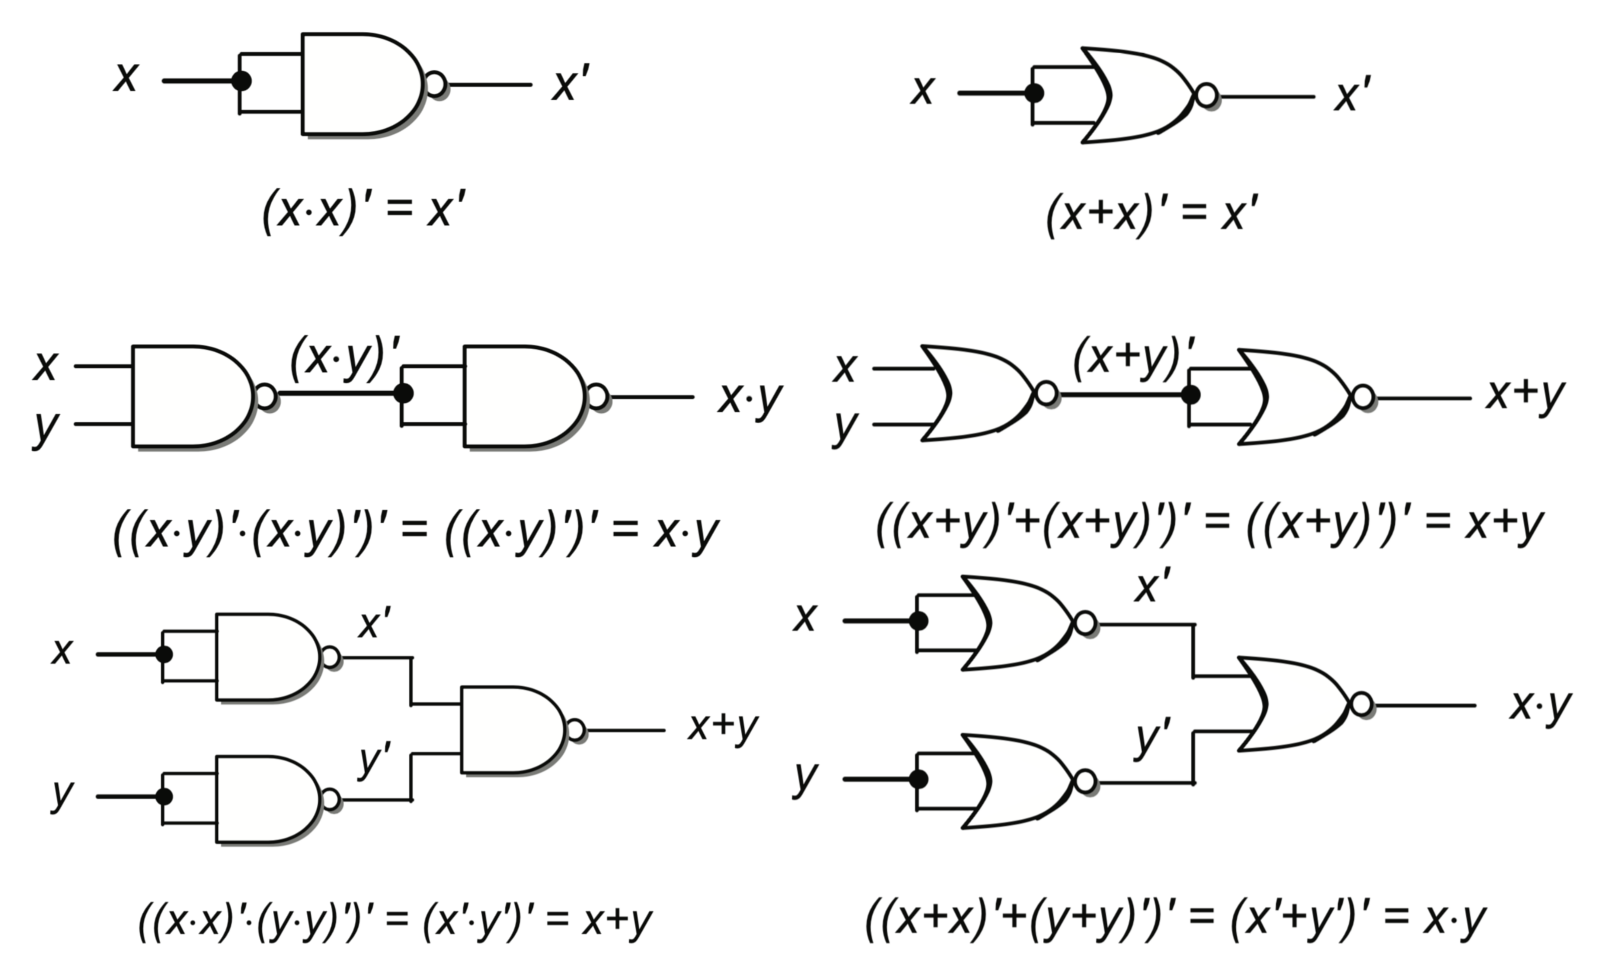
\includegraphics[scale=0.12]{nor_nand}}

\textbf{K-maps}
\begin{itemize}[leftmargin=*]
\itemsep -0.5em
\item Prime Implicant (PI) is a product term formed by combining the {\i maximum} possible no. of minterms (largest group)
\item Essential Prime Implicant (EPI) is a PI that includes at least one minterm not covered by any other group
\item Label the K-map rows/columns in a {\i gray code} manner e.g $00, 01, 11, 10$
\item Grouping $2^N$ cells(only power-sizes are allowed) eliminates n variables
\item EPIs are counted only by checking 1s, {\bf not} $X$s
\item K-maps help to obtain canonical SOP, but might not provide the simplest expression possible (need to use boolean algebra for that)
\end{itemize}

\textbf {Delays} : Note that for combinatorial circuits, there is a delay: for every logic gate with $n$ inputs, calculate $delay = max(t_1, t_2, \dots t_n) + t_delay$
\begin{center}
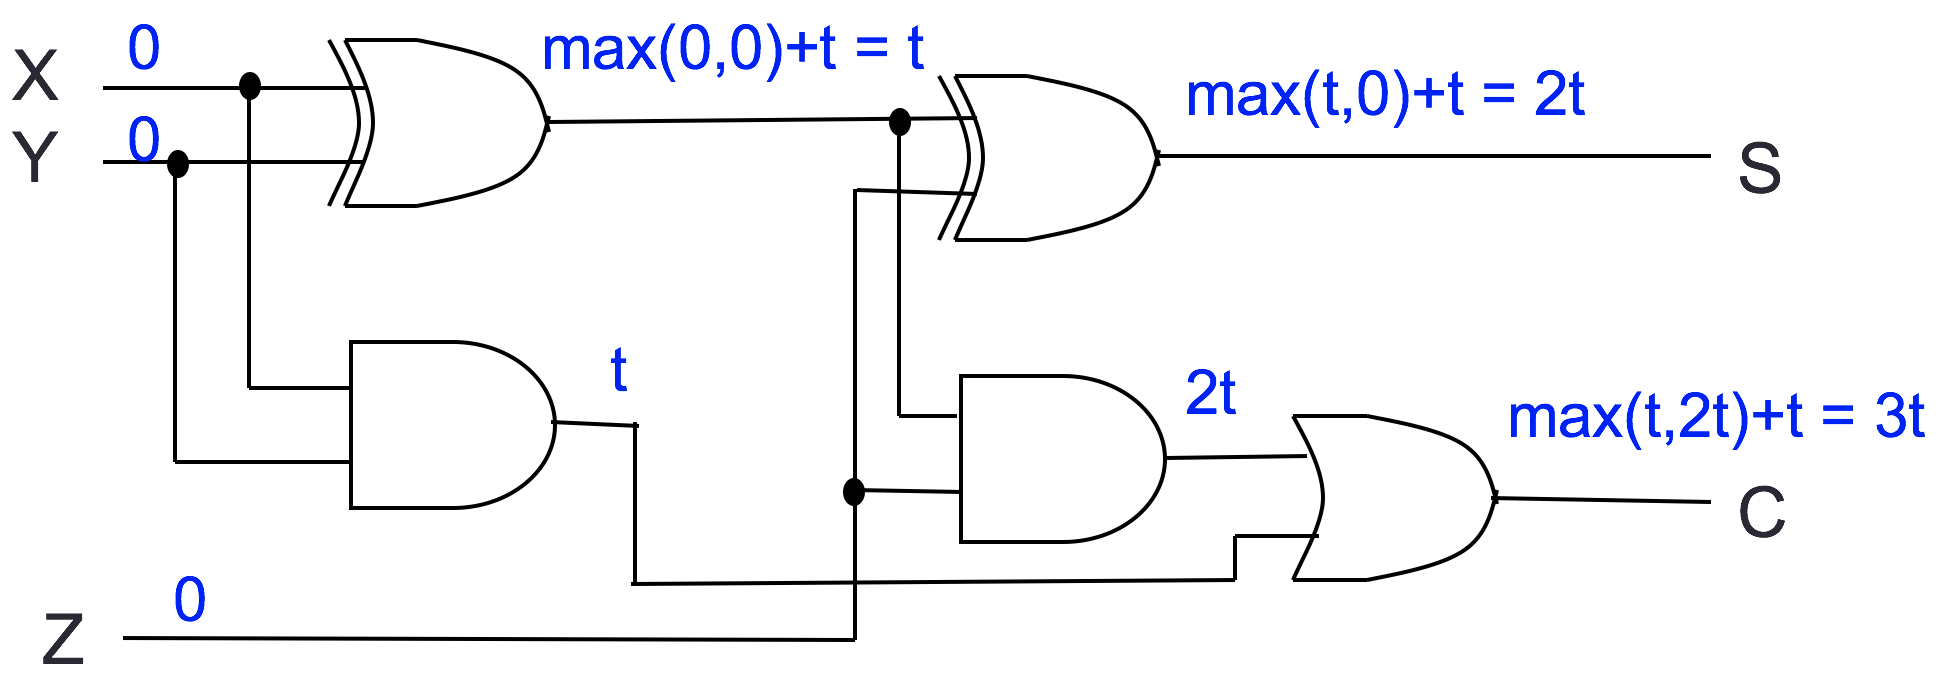
\includegraphics[scale=0.18]{circuit_delay}
\end{center}

\columnbreak
%MSI COMPONENTS%
{\small\textbf{MSI Components}}

\begin{multicols*}{2}
\textbf{{Multiplexer}}
\\ Use minterm as selection line, using 0/1 as inputs. For smaller size multiplexer, use one of the variables for input lines.
\vfill\null
\columnbreak
{\centering 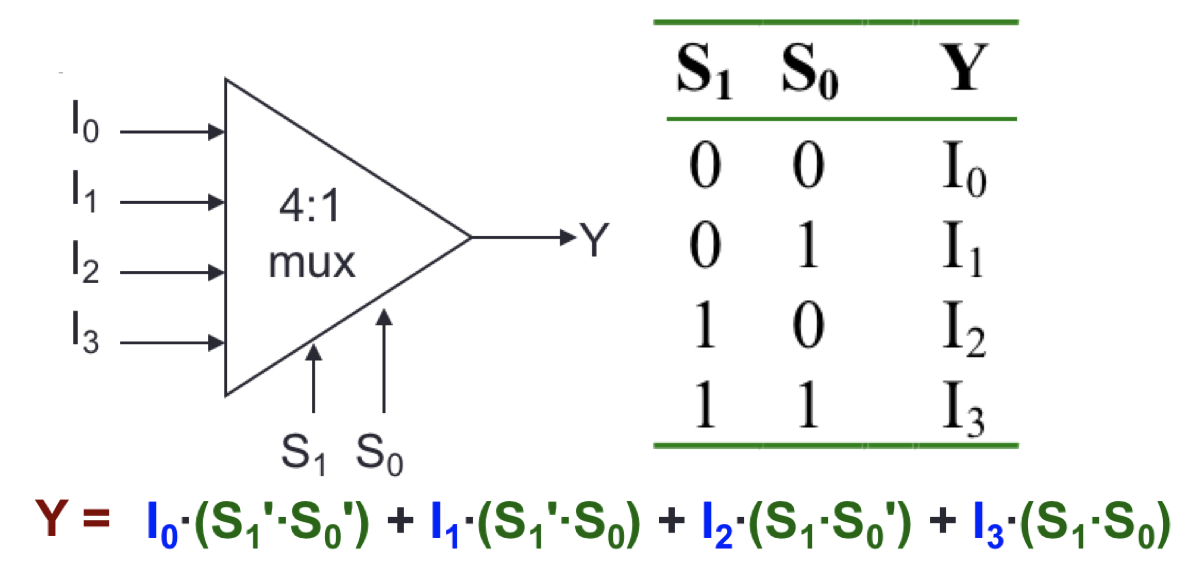
\includegraphics[scale=0.16]{multiplexer}}
\end{multicols*}

\begin{multicols*}{2}
\textbf{{Demultiplexer}}
\vfill\null
\columnbreak
{\centering 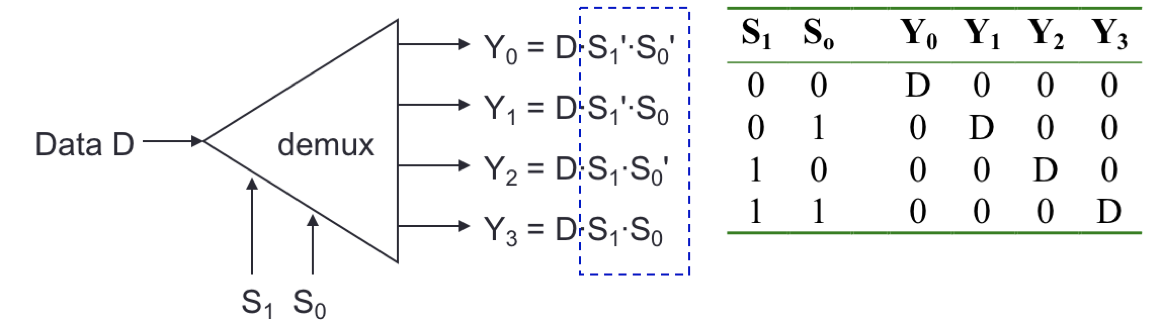
\includegraphics[scale=0.16]{demultiplexer}}
\end{multicols*}

\begin{multicols*}{2}
\textbf{{Encoder}}
\vfill\null
\columnbreak
{\centering 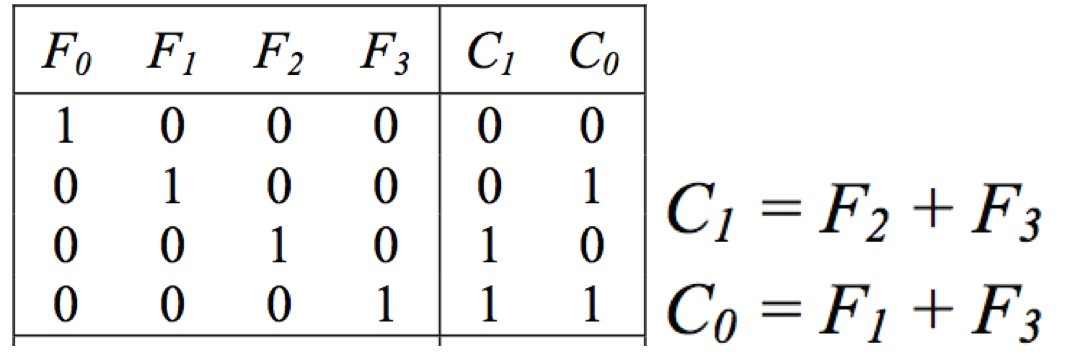
\includegraphics[scale=0.18]{encoder}}
\end{multicols*}

\begin{multicols*}{2}
\textbf{{Decoder}}
\\ Generate minterms and use OR to form a function
Alternatively, use NOR on maxterms.
\vfill\null
\columnbreak
{\centering 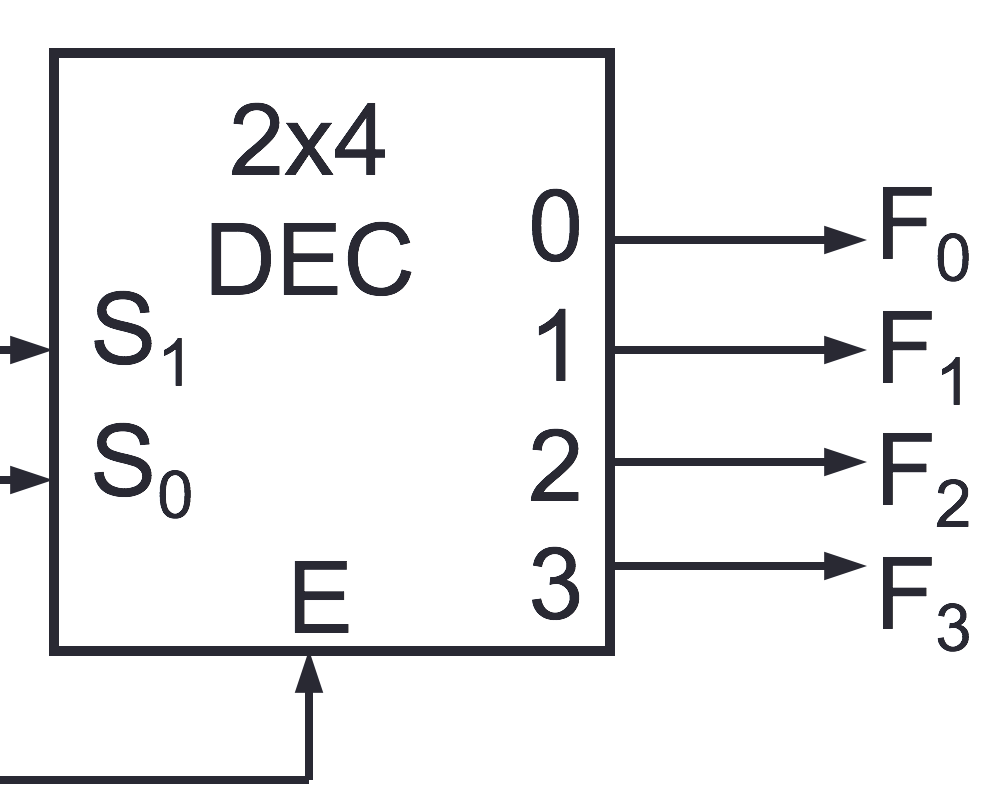
\includegraphics[scale=0.13]{decoder}}
\end{multicols*}

\begin{multicols*}{2}
\textbf{{Priority Encoder}}
\vfill\null
\columnbreak
{\centering 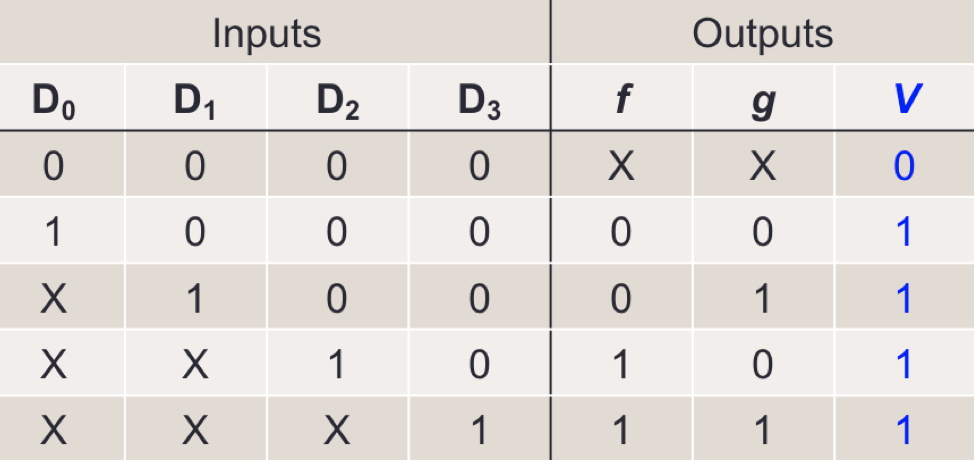
\includegraphics[scale=0.17]{priorityEncoder}}
\end{multicols*}

\begin{multicols*}{2}
\textbf{{Larger Components}}
\\ Remove a decoder that gives duplicate outputs (w.r.t another decoder) by using an OR gate with the outputs from the first decoder, and the enable input of the second.
\vfill\null
\columnbreak
{\centering 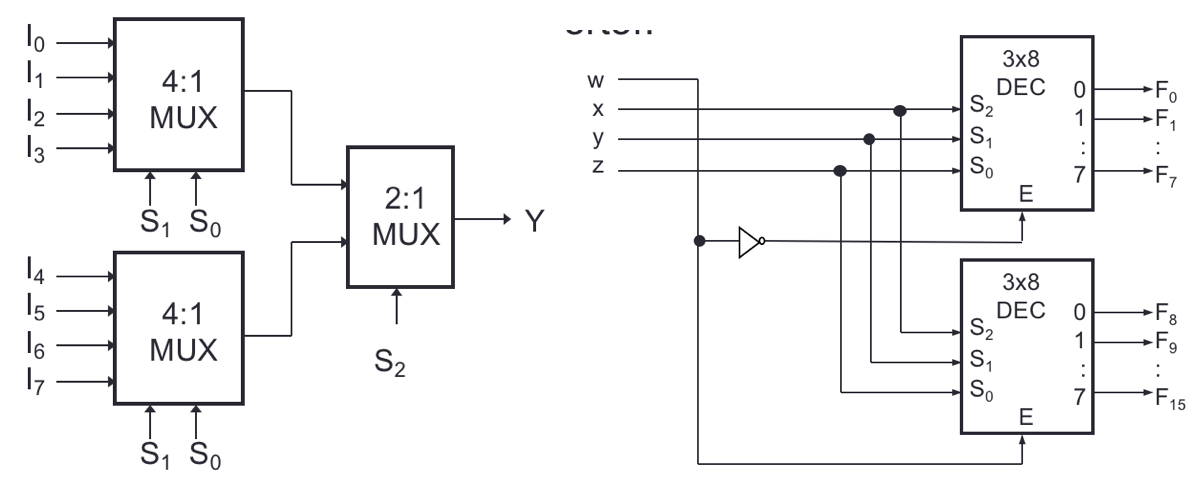
\includegraphics[scale=0.15]{largerComponents}}
\end{multicols*}

%SEQUENTIAL LOGIC%
{\small\textbf{Sequential Logic }}
\\ \textbf{{Excitation Tables}}
\\ {\centering 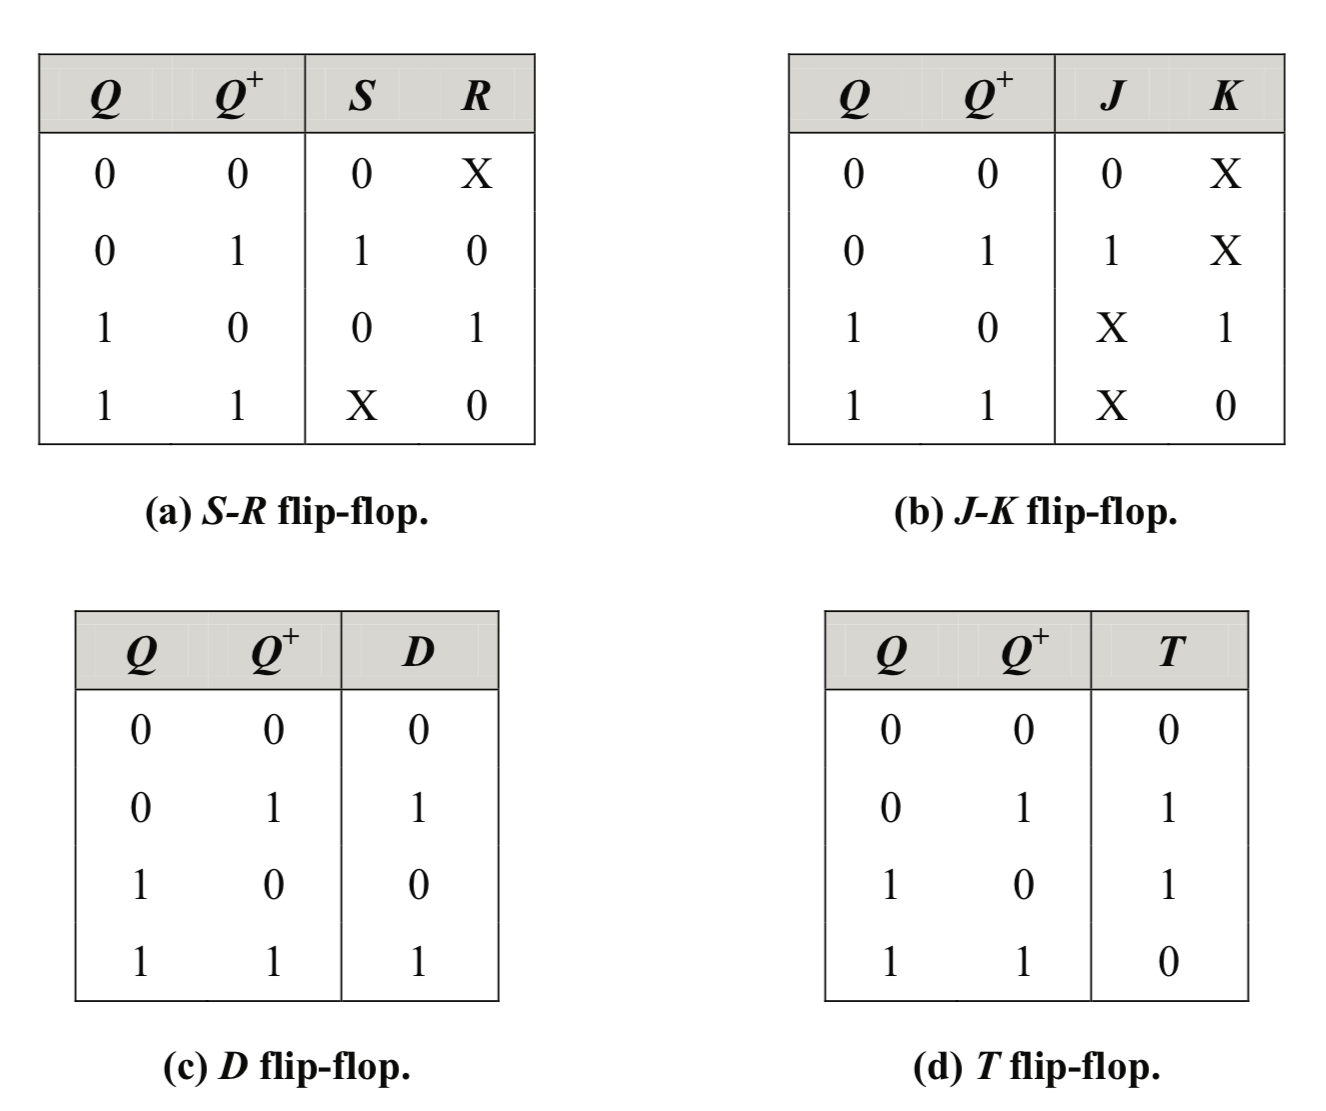
\includegraphics[scale=0.10]{excitationTables}}
\begin{itemize}[leftmargin=*]
\itemsep -0.5em
\item For $m$ flip-flops, up to $2^m$ states exist.
\item SR has invalid code while JK uses that for the toggle code
\item T is the {\i toggle} flip-flop
\item D is the {\i setting} flip-flop
\item Negative input for $Clock$ $\rightarrow$ flip-flop is negative edge-triggered
\end{itemize}

\textbf{{Static RAM}}
\\ {\centering 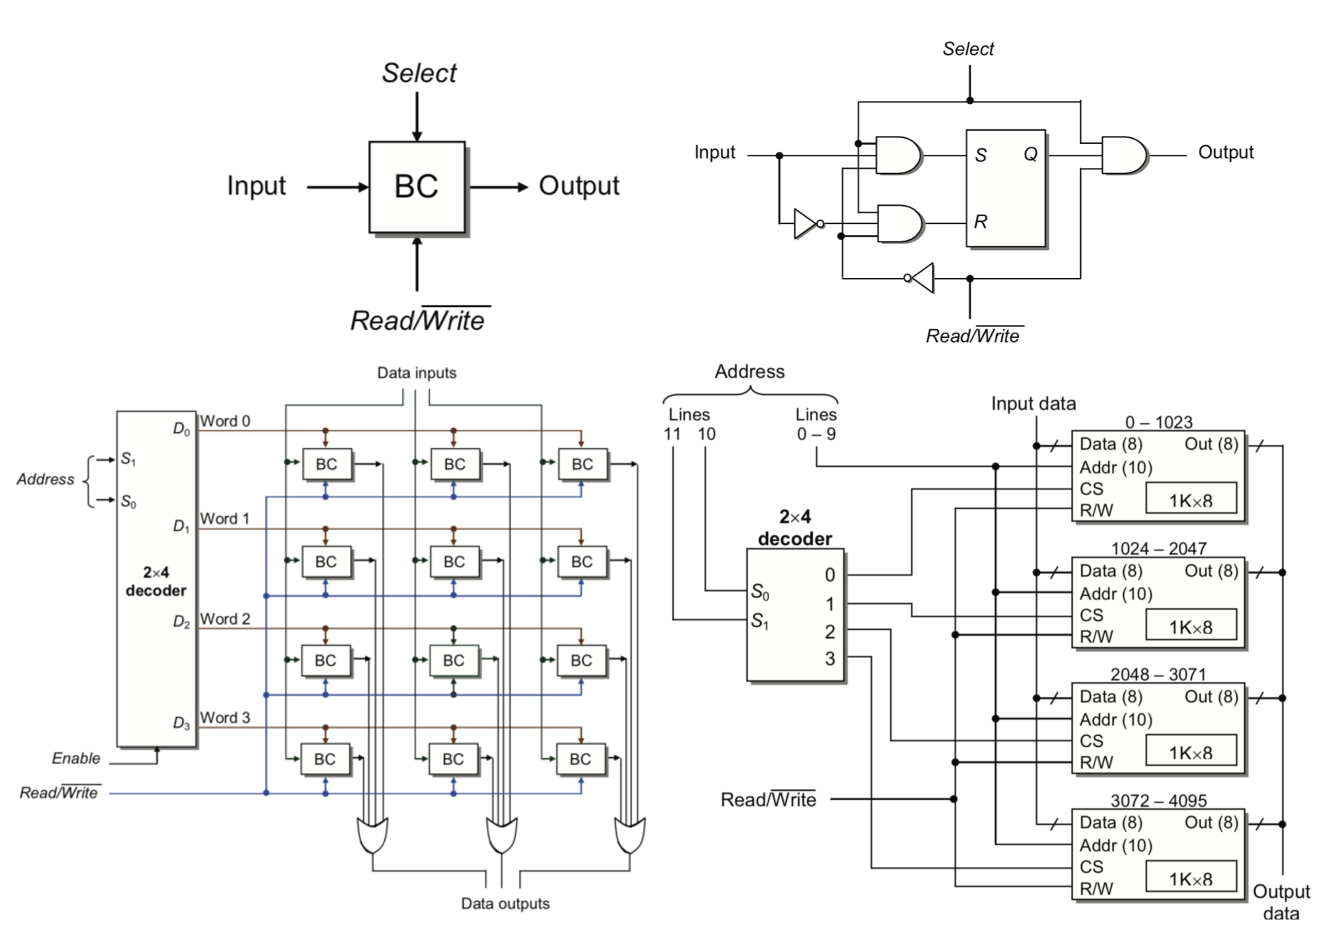
\includegraphics[scale=0.13]{staticRAM}}
\begin{itemize}[leftmargin=*]
\itemsep -0.5em
\item Dyanmic RAM does not use flip-flop as cells
\item For BC, Write is 0, Read is 1 
\item 1K*8 RAM $\Rightarrow$ 1024words*8bits
\item In 12 bit address to 4K*8 RAM constructed using 1K*8 blocks, the 2 most significant bits are fed into decoder to determine which block to use. 
\item Expand horizontally to increase word size, vertically to increase memory size
\end{itemize}


%PIPELINING%
{\small\textbf{Pipelining}}
\\ \textbf{{Pipeline register contents}}
\begin{itemize}[leftmargin=*]
\itemsep -0.5em
\item $IF/ID$: Instruction from memory \& $PC + 4$
\item $ID/EX$: Data read from regsiter files, 32-bit Sign extended $Imm$, \& $PC + 4$
\item $EX/MEM$: $Imm$, \& $(PC + 4) + (Imm * 4)$, ALU result, $isZero$ signal \& $RD2$ from register file
\item $MEM/WB$: ALU result, Memory read data \& write regsiter data (passed through all pipelines)
\end{itemize}

\textbf{{Performance}}
\begin{itemize}[leftmargin=*]
\itemsep -0.3em
\item If cycle/clock time is given, just use that 
\item Single cycle: 
    \\ $CT_{seq} = \sum^N_{k=1}T_k$
    \\ $Time_{seq}  = I * CT_{seq}$ (choose the maximum $CT_{seq}$)
\item Multi-cycle [1 stage per cycle, cycle time chosen to be time for longest stage]
    \\ $CT_{multi} = max(T_k)$ i.e longest stage time
    \\ $Time_{multi} = I * Average CPI * CT_{multi}$ 
\item Pipeline [Several stages per cycle]
    \\ $CT_{pipeline} = max(T_k) + T_d$ where $T_d$ is the pipeline register overhead 
    \\ $Time_{pipeline} = (I + N - 1) * CT_{pipeline}$ 
\item If $N_{intstructions} >> N_{stages}$, 
    \\ $Speedup_{pipeline} = \frac{Time_{seq}}{Time_{pipeline}}$
\end{itemize}

\textbf{{Hazard and resolution}}
\begin{itemize}[leftmargin=*]
\itemsep -0.5em
\item Without data forwarding: If dependent cycle is
    \\ $\cdot$ right before: 2 cycle delay
    \\ $\cdot$ 2 cycles before: 1 cycle delay
\item With data forwarding: If dependent cycle is
    \\ $\cdot$ dependent on lw: 1 cycle delay
    \\ $\cdot$ otherwise: no delay
\item Without control measures: 3 cycle delay 
\item With early branching/resolution: 1 cycle delay after branch instruction  
    \\ $\cdot$ with forwarding \& dependent on non-lw: 1 cycle bef branch
    \\ $\cdot$ with forwarding \& dependent on lw: 2 cycles bef branch 
    \\ $\cdot$ without forwarding: dependent: 2 cycle delay bef branch 
\item With branch prediction: 
    \\ $\cdot$ 3 cycles occur if no early branching
    \\ $\cdot$ 1 cycle occur if there is early branching
    \\ $\cdot$ then, instructions either get flushed/not flushed
\item With delayed branch: If $\exists$ instruction before branch that can be moved into delayed slot, move it. Else, stall/no-op
\end{itemize}

%CACHE%
{\small\textbf{Cache}}
\\ \textbf{{Average Access time}}
\\ $Rate_{hit} * Time_{hit} + (1 - Rate_{hit}) * Penalty_{miss}$

\textbf{{Direct Mapped Cache}}
\begin{itemize}[leftmargin=*]
\itemsep -0.5em
\item Blocks in cache: $2^M$
\item Bytes per block: $2^N$
\end{itemize}

\textbf{{Set Associative Cache}}
\begin{itemize}[leftmargin=*]
\itemsep -0.5em
\item $N$-way SAC $\rightarrow$ $N$ cache blocks per set
\item Bytes per block: $2^M$
\item Cache bocks = $\frac{Size_{cache}}{Size_{block}}$
\item Sets = $\frac{CacheBlocks}{N}$ = $2^N$
\end{itemize}

\textbf{{Fully Associative Cache}}
\begin{itemize}[leftmargin=*]
\itemsep -0.5em
\item Bytes per block: $2^N$
\end{itemize}

\textbf{{For each address}}
\begin{itemize}[leftmargin=*]
\itemsep -0.5em
\item Set Index =  $(val \bmod 2^{N + M}) // 2^N$
\item Word Index =  $(val \bmod 2^{N}) // Bytes_{word}$
\item Tag =  $val // 2^{N + M}$
\end{itemize}

\textbf{{Miss Rates}}
\begin{itemize}[leftmargin=*]
\itemsep -0.5em
\item Conlfict miss rates decrease with increasing associativity
\item DMC of size $N$ has the same miss rate as a 2-way SAC of size $\frac{N}{2}$
\item Capacity miss only depends on cache size, same size $\rightarrow$ same capcatiy miss
\item As cache size increases, capcacity miss decreases
\end{itemize}

\textbf{{Block Replacement}}
\begin{itemize}[leftmargin=*]
\itemsep -0.5em
\item Least Recently Used: Note that it is hard to keep track if there are many choices and there is a cost to keeping track of this as well
\item First in First out
\item Random Replacement
\item Least Frequently Used
\end{itemize}

\textbf{{Writing Policy}}
\begin{itemize}[leftmargin=*]
\itemsep -0.5em
\item Write through cache: Write to both cache and main memory
\item Write back cache: Only write to cache, write to memory when block is replaced
\item Write Miss -- Write allocate: Load complete block and write onto the cache $\Rightarrow$ Write to main memory if using write through policy
\item Write Miss -- Write around: Do not load block to cache, write to memory only
\end{itemize}

% DIAGRAMS %
\vfill\null
\columnbreak
\begin{center}
{\centering 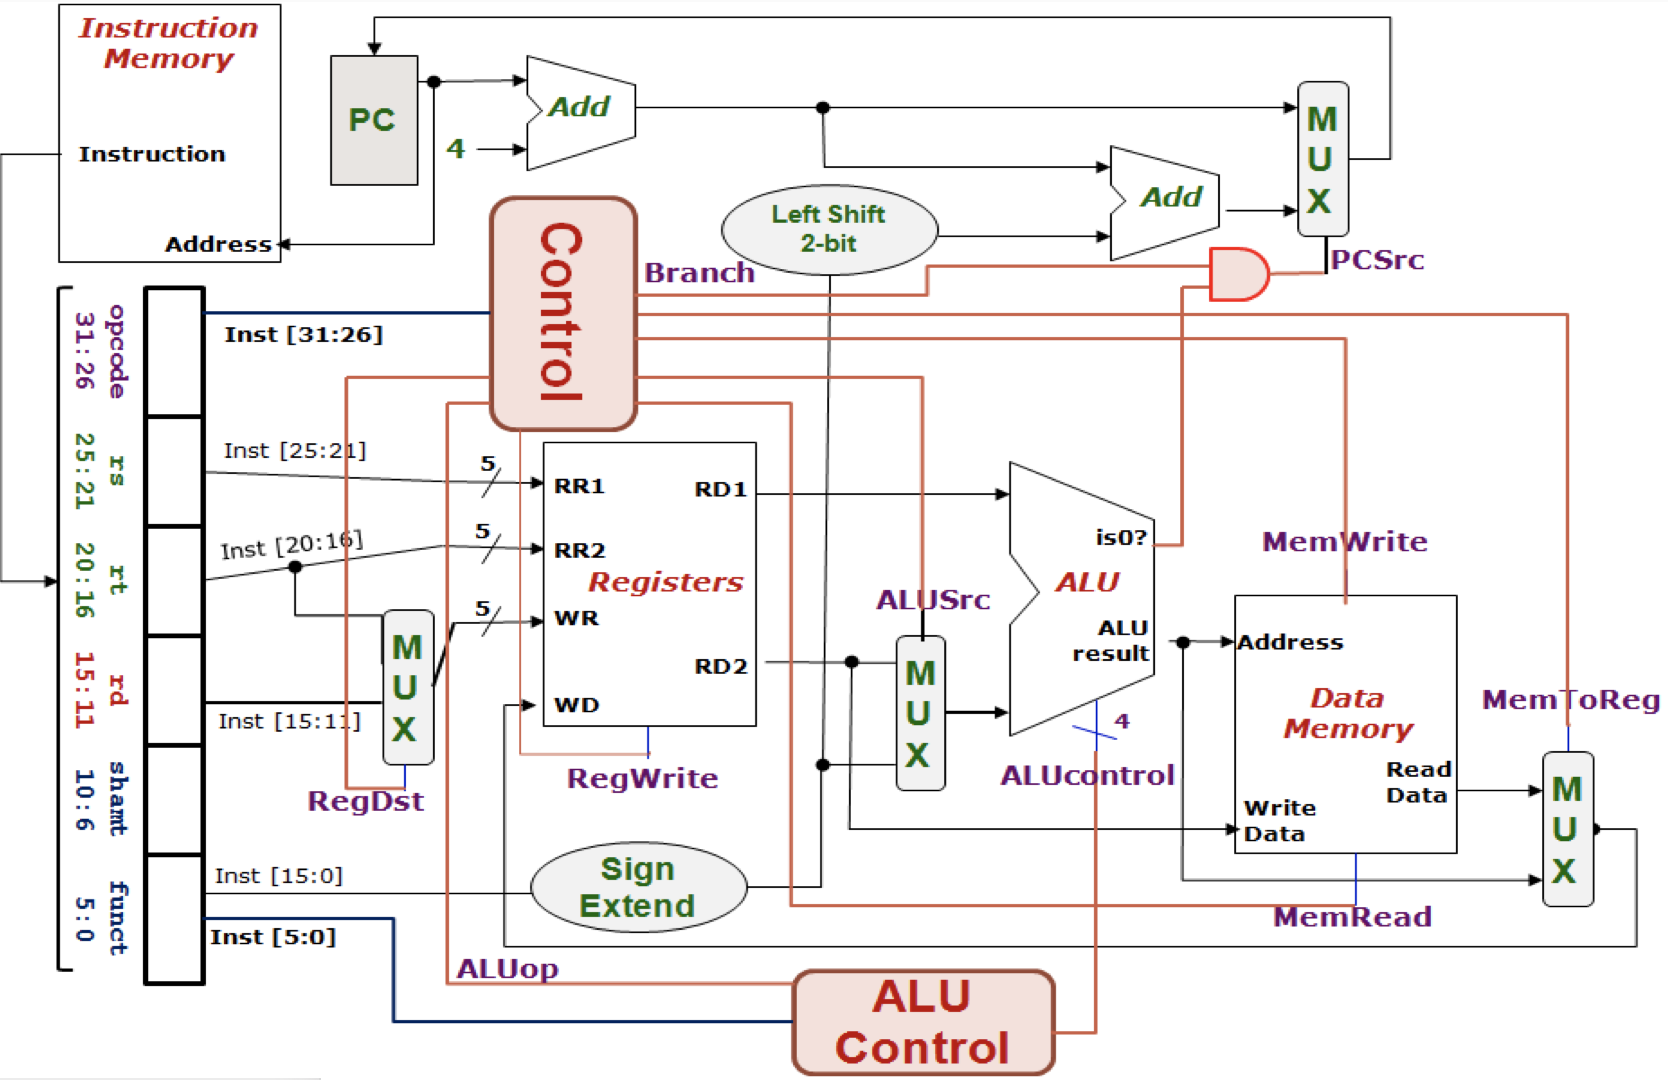
\includegraphics[angle=90,origin=c,scale=0.35]{dataPath}}
\\ {\centering 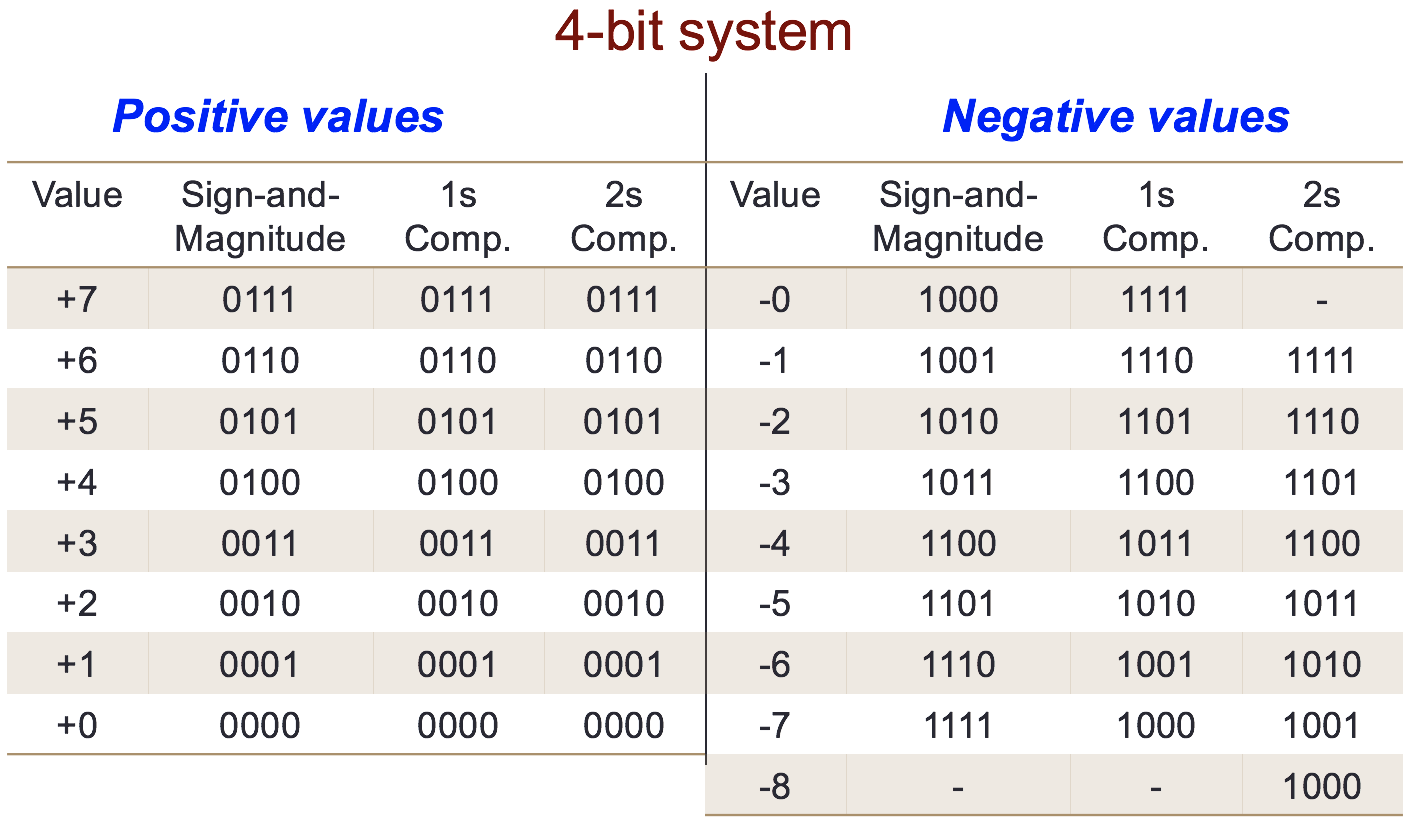
\includegraphics[angle=90,origin=c,scale=0.30]{fourBitRepresentation}}
{\centering 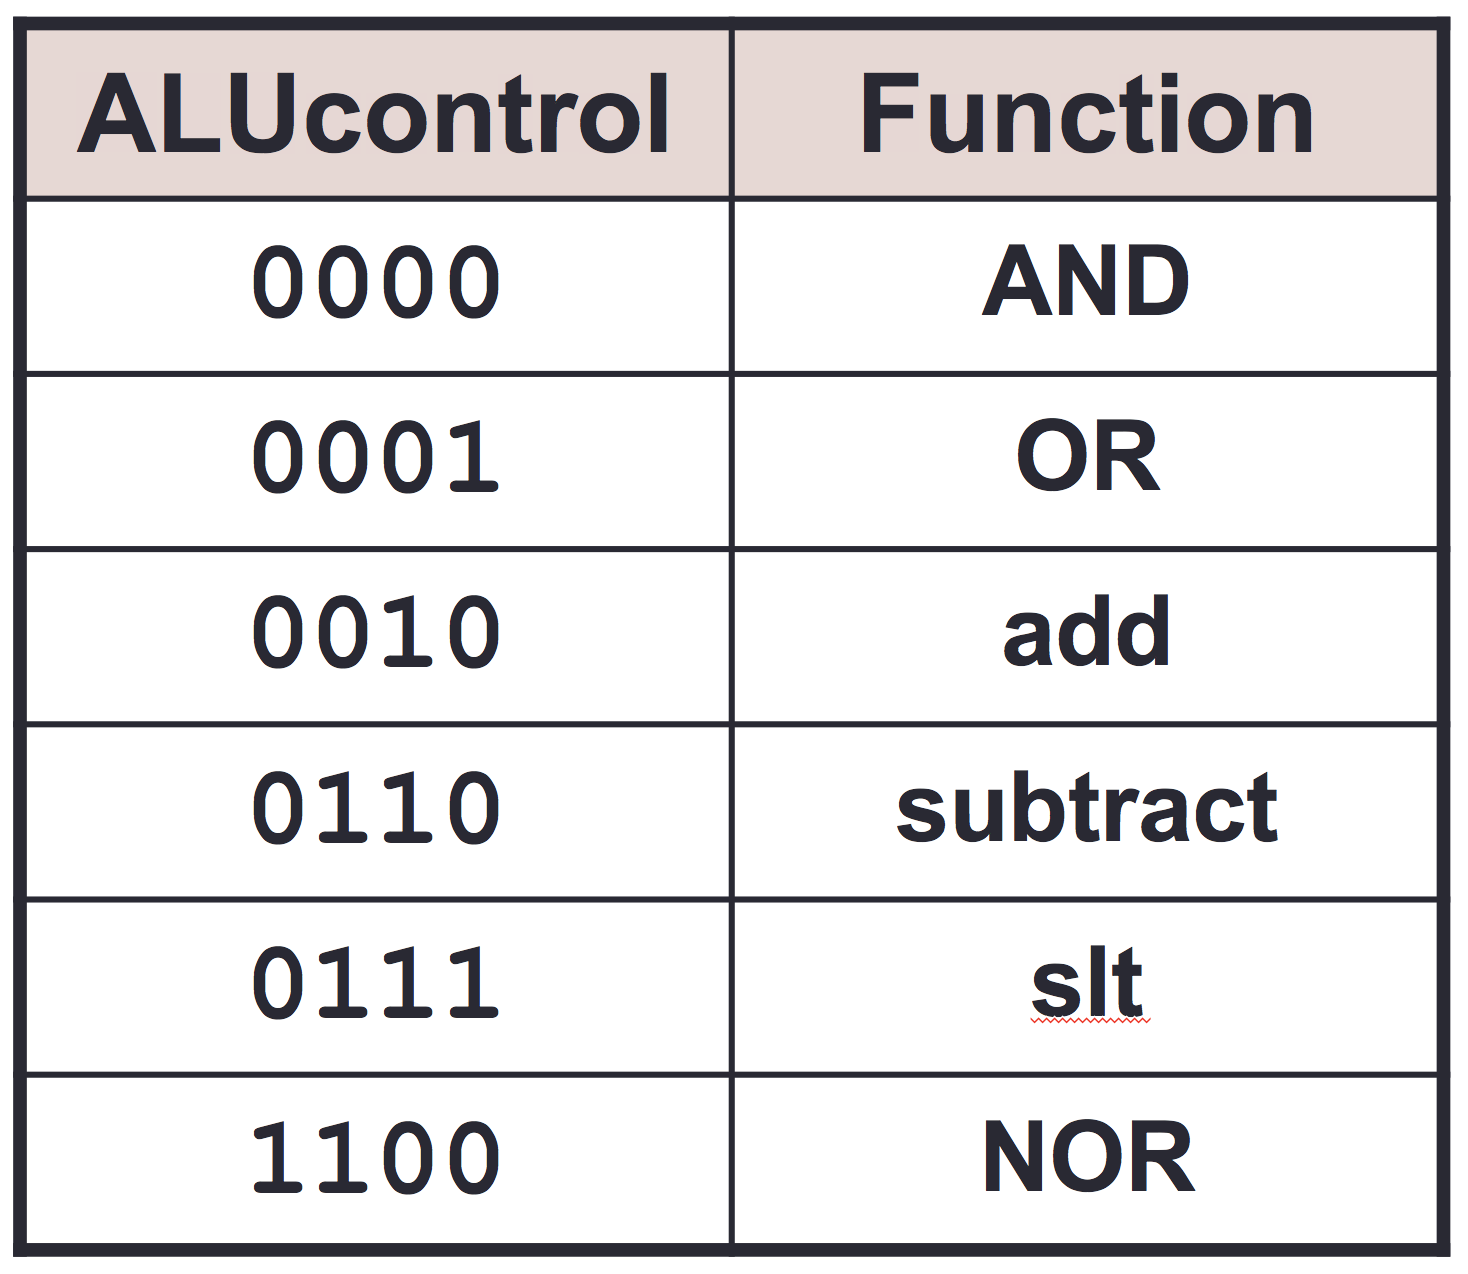
\includegraphics[scale=0.13]{ALUControl}}
\\ {\centering 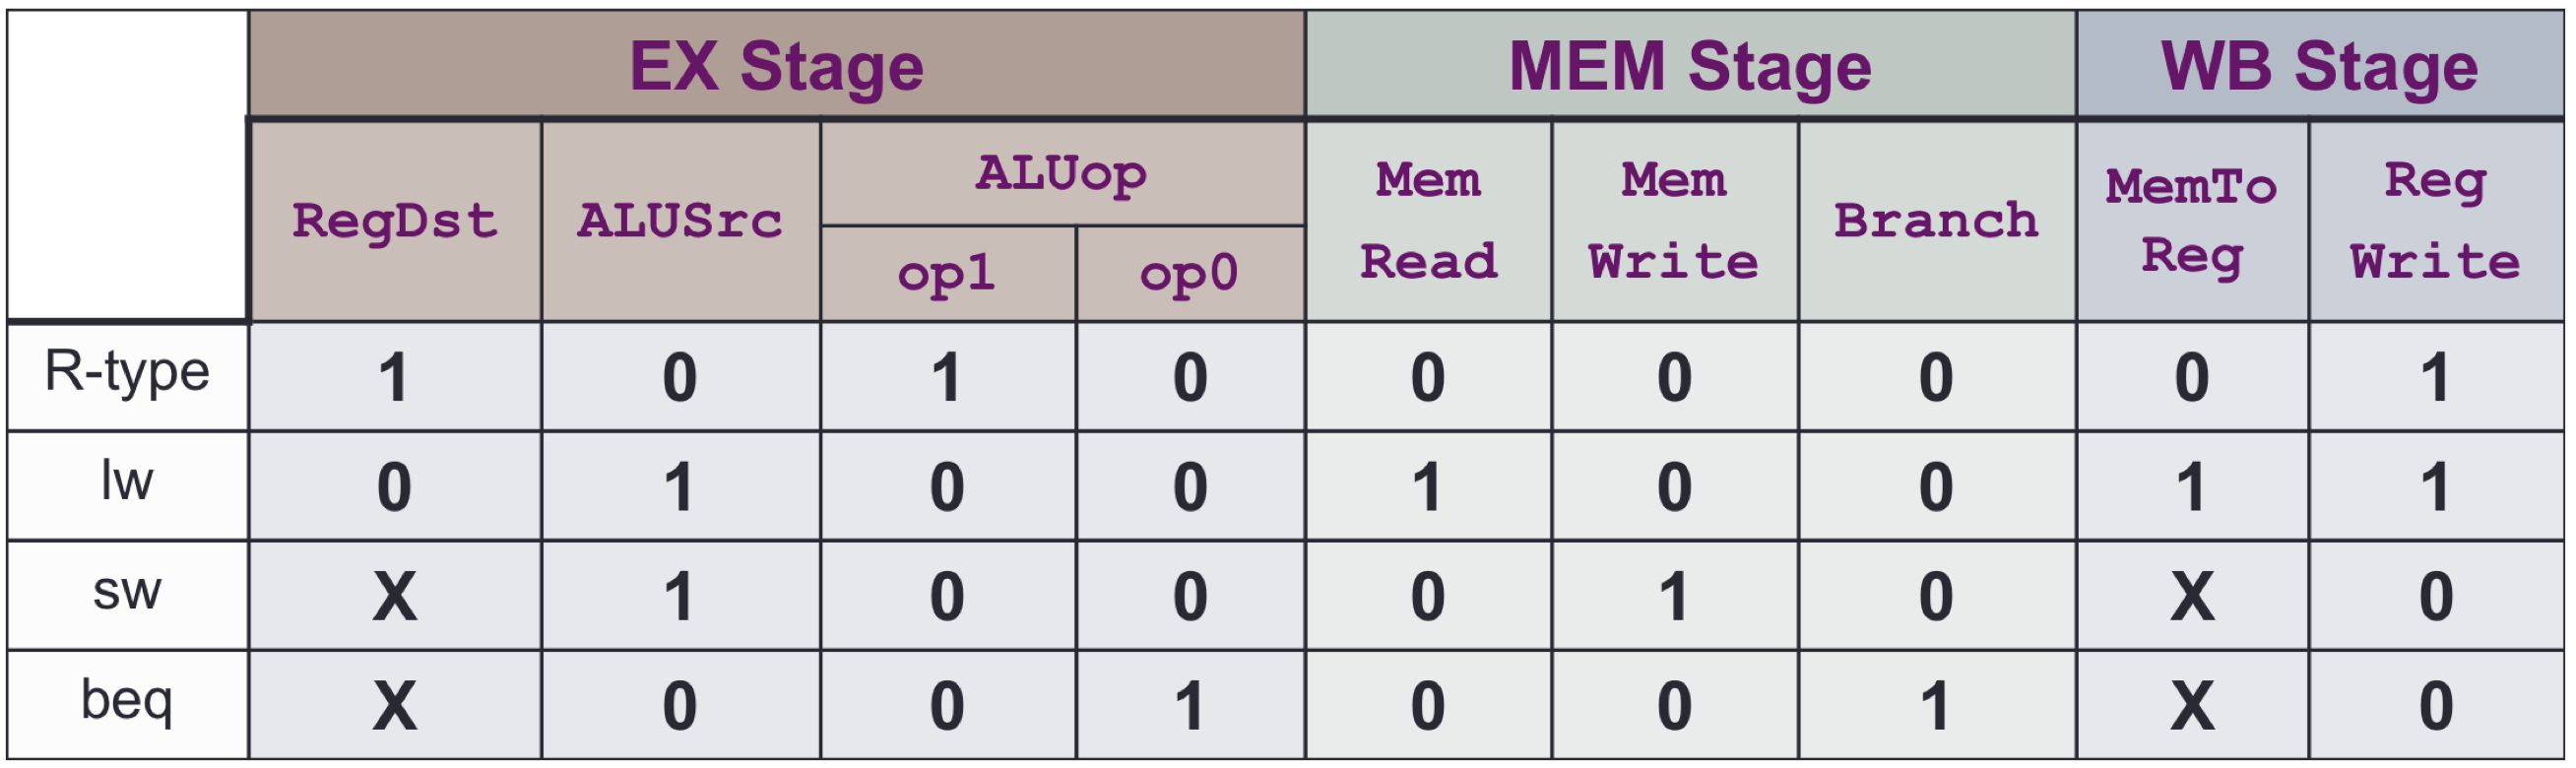
\includegraphics[angle=90,origin=c,scale=0.25]{instructionControl}}
{\centering 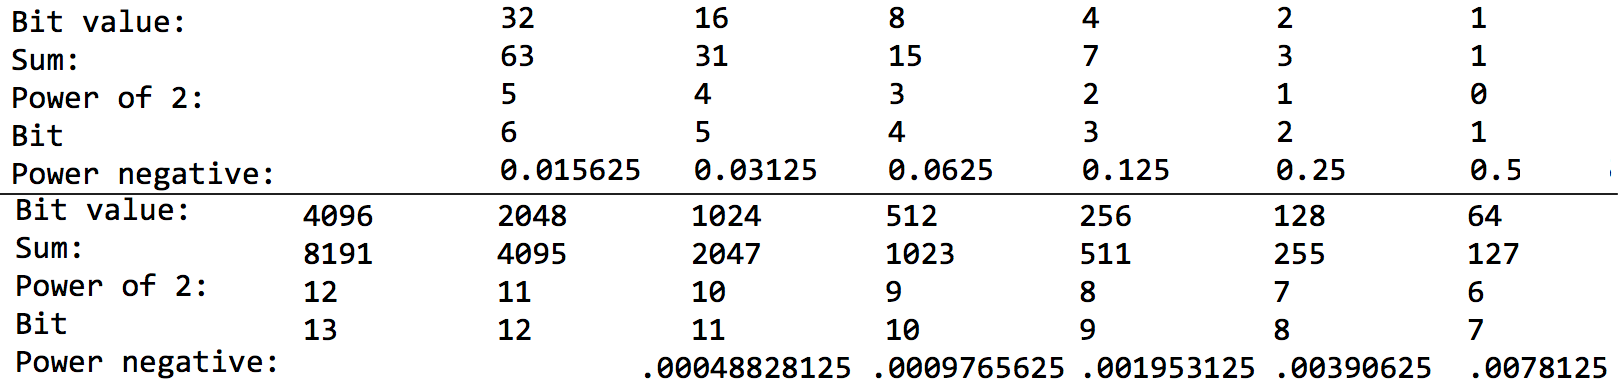
\includegraphics[angle=90,origin=c,scale=0.34]{powersOfTwo}}
\vspace{5mm} %5mm vertical space
\\ {\centering 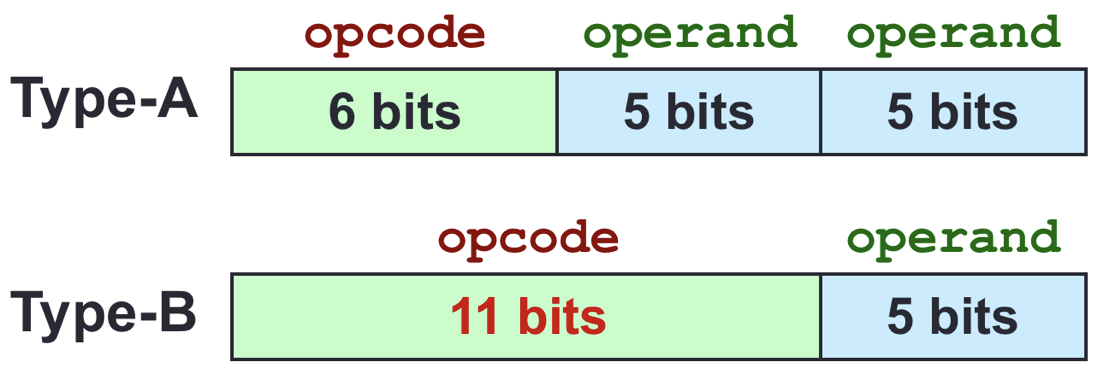
\includegraphics[scale=0.25]{expandingOpcode} }
\\ Max (1 type A) = $1 + (2^6 - 1) * 2^5$
\\ Min (1 type B) = $(2^6 - 1) + 2^5$

\vspace{5mm} %5mm vertical space
\begin{tabular}{ |c c| } 
 \hline
 Input & 0X DE AD BE EF  \\ 
 Big-Endian & 0: DE, 1: AD \dots  \\ 
 Little-Endian & 0: EF, 1: BE \dots  \\ 
 \hline
\end{tabular}
\end{center}

    \end{multicols*}
\end{document}
